\documentclass{easychair}

\title{A note on conflict set generation\\ for congruence closure\\\small Extended abstract}
\titlerunning{A note on congruence closure}

\author{Andreas Fellner\inst{1,2}
   \and Pascal Fontaine\inst{3}
   \and\\ Georg Hofferek\inst{4}
   \and Bruno Woltzenlogel Paleo\inst{2,5}
}
\institute{IST-Austria, Klosterneuburg (Austria)
\and Vienna University of Technology (Austria)
\and Inria, Loria, U. of Lorraine (France)
\and IAIK, Graz University of Technology (Austria)
\and Australian National University and NICTA (Australia)
}

\authorrunning{Fellner et al.}

\usepackage{amssymb}
\usepackage{graphicx}            			% Figures
\usepackage{tikz}					% tikz graphics
\usetikzlibrary{arrows,automata,positioning}
\usetikzlibrary{fit}
%\usepackage{hyperref}

\newtheorem{example}{Example}
\newtheorem{definition}{Definition}
\newtheorem{corollary}{Corollary}
\newtheorem{theorem}{Theorem}
\newtheorem{lemma}{Lemma}

\begin{document}

\maketitle

\begin{abstract}
The efficiency of Satisfiability Modulo Theories (SMT) solvers is dependent on
the capability of theory reasoners to provide small conflict sets, i.e.\ small
unsatisfiable subsets from unsatisfiable sets of literals.  Decision procedures
for uninterpreted symbols (i.e.\ congruence closure algorithms) date back from
the very early days of SMT.  Nevertheless, to our best knowledge, the complexity
of the smallest conflict set generation for sets of literals with uninterpreted
symbols and equalities had not yet been determined, although it is believed to
be NP-complete.  We provide here an NP-hardness proof, using a simple reduction
from SAT.
\end{abstract}


\section*{Introduction}

Satisfiability Modulo Theory solvers are nowadays based on a cooperation of a
propositional satisfiability (SAT) solver and a theory reasoner for the
combination of theories understood by the SMT solver. The propositional
structure of the problem is handled by the SAT solver, whereas the theory
reasoner only has to deal with conjunctions of literals.  Very schematically (we
refer to~\cite{Barrett14} for more details) the Boolean abstraction of the SMT
problem is repeatedly refined by adding theory conflict clauses that eliminate
spurious models of the abstraction, until either unsatisfiability is reached, or
a model of the SMT formula is found.  Refinements can be done by refuting models
of the propositional abstraction one at a time.  It is, however, much more
productive to refute all propositional models that are spurious for the same
reason.  A model of the abstraction is spurious if the set of concrete literals
corresponding to the abstracted literals satisfied by this model is
unsatisfiable modulo the theory.  Given such an unsatisfiable set of concrete literals, the
disjunction of the negations of any unsatisfiable subset (a.k.a. \emph{core}) is a suitable
conflict clause.  By backtracking and asserting the conflict clause, the
SAT-solver is prevented from generating the spurious model again. The smaller
the clause, the stronger it is and the more spurious models it prevents.
Therefore, an optimal conflict clause, corresponding to a minimal unsatisfiable
subset of literals (i.e.\ such that all its proper subsets are satisfiable) or
even a minimum one (i.e.\ smallest among the minimals) is desirable.  This
feature of the theory reasoners to \emph{generate small conflict sets} (a name
adopted in~\cite{Barrett14}) from their input is also referred by \emph{proof
production}~\cite{Nieuwenhuis3,Nieuwenhuis9} or \emph{explanation
generation}~\cite{Nieuwenhuis6}.
%% \marginpar{TODO: This footnote is vague. I would suggest removing it. ``unuseful'' doesn't exist, but ``useless'' would sound too strong. }\footnote{\emph{Proof production} and \emph{explanation
%%   generation} additionally convey the idea that, besides giving a small
%%   unsatisfiable subset, the valuable reasoning process can be isolated from the
%%   unuseful computation.}

Decision procedures for the theory of uninterpreted symbols and equality can be
based on congruence closure~\cite{Nelson2,Downey1,Nieuwenhuis6}.  The decision problem is polynomial
and even quasi-linear~\cite{Downey1} with respect to the number of terms and
literals in the input set.  Producing minimal conflict sets also takes
polynomial time.  Indeed, testing if a set $S$ remains unsatisfiable after
removal of one of its literal is also polynomial.  It suffices then to
repeatedly test the $|S|$ literals of $S$ to check if they can be removed.  The
set $S$ pruned of its unnecessary literals is minimal.  One can also make profit of the incrementality of the decision procedure~\cite{Fontaine1}.

It has also been common knowledge that computing minimum conflict clauses for
the theory of uninterpreted symbols and equality is a difficult problem.  But,
to our best knowledge, the complexity of the smallest conflict clause generation
for sets of literals with uninterpreted symbols and equalities has never been
established.  It is mentioned to be NP-complete in~\cite{Nieuwenhuis8} --- with
a reference to a private communication with Ashish Tiwari --- but neither the
authors of~\cite{Nieuwenhuis8} nor Ashish Tiwari published a written proof of
this fact\footnote{We contacted both Ashish Tiwari and the authors
  of~\cite{Nieuwenhuis8} who confirmed this.}.

Our interest in this problem arose from our work on Skeptik \cite{Boudou1}, a tool for the compression of proofs generated by SAT and SMT solvers. For the sake of moving beyond the purely propositional level, we have developed an algorithm for compressing congruence closure proofs, which consists of regenerating (possibly smaller) congruence closure conflict clauses while traversing the proof. Congruence closure conflict clauses are typically generated from paths in the \emph{congruence graph} maintained by the congruence closure algorithm \cite{Fontaine2004,Nieuwenhuis6,Nieuwenhuis9}. During the replay, we use a polynomial-time algorithm for searching for short paths in the congruence graph, which is a modification of Dijkstra's shortest path algorithm \cite{Dijkstra1959}. This raised the question whether our algorithm could find the shortest conflict clauses, as Dijkstra's algorithm finds shortest paths. We answered this question negatively by proving that the problem of deciding whether a shorter conflict clause exists is NP-hard. The goal of this short note is to present this proof.

\section*{Notations}

We assume knowledge of propositional logic and quantifier-free first order logic
with equality and uninterpreted symbols.  We only enumerate the notions and
notations used in this paper.
%TODO Propositional logic studies formulas written  $\vee$, $\wedge$, $\neg$
A literal is either a propositional variable or the negation of a propositional
variable.  A clause is a disjunctive set of literals.  A propositional variable
$x$ appears positively (negatively) in a clause $C$ if $x \in C$ (resp.\ $\neg x
\in C$).  The notations $\{\ell_1, \dots \ell_n\}$ and $\ell_1 \vee \dots
\ell_n$ will be used interchangeably.  A formula in conjunctive normal form (CNF
for short) is a conjunctive set of clauses.  A total (partial) assignment $\cal
I$ for a formula in propositional logic associates a value in $\{\top, \bot\}$
to every (resp.\ some) propositional variable in the formula.  An assignment
$\cal I$ for a formula $F$ is a model of $F$, noted ${\cal I}\models F$, if it makes
the formula $F$ true.  A formula is satisfiable if it has a model, it is
unsatisfiable otherwise.  A total or partial assignment can be perfectly
defined by the set of literals it makes true.  By default, an assignment is
total unless explicitly said to be partial.

We use the usual notions of (un)satisfiability and model also for
quantifier-free first-order logic.  A constant is a nullary function.  For
convenience, we will use notations like $\top_i$ and $\bot_i$ as constants, with
no implicit relation to the Boolean constants $\top$ and $\bot$.  A set of
formula $E$ entails a (set of) formula(s) $E'$, denoted $E\models E'$, if every
model of $E$ is a model of $E'$.

\vspace*{5pt}
\noindent \textbf{Congruence closure and congruence graph}

\noindent
We do not give here a full description of congruence closure algorithms and
refer the reader to~\cite{Nelson2,Downey1,Nieuwenhuis6} for more details.  We
only remind that the satisfiability of a set of first-order literals with
equality and uninterpreted symbols $E$ can easily be checked by building a
congruence graph.  A congruence graph is built on a set of nodes including (but
not restricted to) all terms and subterms in $E$.  We assume this set of nodes
is finite, and unless stated otherwise, only contains the terms and subterms in
$E$.  There are two kinds of edges in the graph: full edges and congruence
edges.  There is a full edge between two nodes associated with terms $s$ and $t$
if and only if there is an equality $s=t$ (or $t=s$) in $E$.  The congruence
closure algorithm adds congruence edges to the graph until (the smallest)
fix-point is reached: a congruence edge is added between two terms with the same
top symbol $f(s_1, \dots s_n)$ and $f(t_1, \dots t_n)$ if there is a path (using
full and congruence edges) from $s_i$ to $t_i$ for all $i\in \{1,\dots n\}$.  An
equality $s=t$ is implied by a set of literals $E$ if and only if there is a
path between $s$ and $t$ in the congruence graph of $E$ built on all terms and
subterms in $E$, $s$ and $t$.  A set of first-order literals $E$ is
unsatisfiable if and only if there is an inequality $s\neq t \in E$ such that
there is a path between $s$ and $t$ in the congruence graph of $E$.

\section*{NP-completeness of small conflict set generation problem}
\label{sec:npcomplete}

\marginpar{We have to find where to put this remark.}
\marginpar{Bruno: one possibility would be to put these remarks after lemma 3. Maybe we should omit these remarks until we fully convert our current results to results using these alternative ways of measuring size of the problem. }  The algorithms we consider here take as input a set of literals $S$.  When we consider complexity, not only the cardinality of the set is important, but also the number of terms and subterms as well as the number of their occurrences.  Congruence closure algorithms in modern SMT solvers also typically work on Directed Acyclic Graphs (DAGs), not on trees to represent terms.  In that case, what matters is not the number of term and subterm occurrences, but only the number of (sub)terms.  However, the input is also typically not a set, but successive call to an assertion function with a literal as argument.  In that case, every repetition of the same literal would count.  Let us assume however here that the input is a set $E$, that terms are DAGs with maximal sharing (identity of two terms can be checked in constant time), and that identity of two function symbols can be checked in constant time.

%% Rather than considering directly the conflict set generation problem ---
%% given a natural number $k$ and an unsatisfiable set of literals, is there a
%% conflict set with size smaller than $k$ --- we will rather work on the small
%% explanation problem: given a natural number $k$ a set of equalities $E$ and
%% an equality $s=t$ is there a subset of $E$ smaller than $k$ that implies a
%% given equality $s=t$.

%Let us first define the small conflict set generation problem formally:

\begin{definition}[Small conflict set generation problem]
Given an unsatisfiable set $E$ of literals in quantifier-free first-order logic
with equality and $k \in \mathbb{N}$, the \emph{small conflict set generation
  problem} is the problem of finding whether there exists an unsatisfiable set
$E' \subseteq E$ with $|E'| \leq k$.
\end{definition}
\noindent This problem is NP-complete.  Our proof reduces the problem
of deciding the satisfiability of a propositional logic formula in conjunctive
normal form (SAT) to the small \emph{explanation problem}:
\begin{definition}[Small explanation problem]
Given a set of equations $E = \{ s_1 = t_1,\ldots, s_n = t_n\}$, $k \in
\mathbb{N}$ and a target equation $s = t$, the \emph{small explanation problem}
is the problem of finding whether there exists a set $E'$ such that $E'
\subseteq E$, $E' \models s = t$ and $|E'| \leq k$.
\end{definition}

\marginpar{In this paragraph, we are assuming that $=$ is the only predicate symbol. But we have not stated this assumption before. }
\noindent The small explanation problem and the small conflict set generation
problem are closely related.  There is a small explanation of size $k$ of $s=t$
from $E$ if and only if there is a small conflict of size $k+1$ for $E \cup
\{s\neq t\}$.  Our proof of hardness is based on a (polynomial) translation of
the propositional satisfiability problem to the small explanation problem.

\newcommand{\Assignment}{{\it Assignment}}
\newcommand{\Clause}{{\it Clause}}
\newcommand{\Connect}{{\it Connect}}

\begin{definition}[CNF congruence translation]

Let $\mathcal{C}$ be a set of propositional clauses $\{C_1,\ldots C_n\}$ using variables $x_1,\ldots,x_m$.
%The set of terms $\mathcal{T}$ is constructed using the following constants and function symbols.
%For every $i= 1,\ldots,n + 1$, there is a constant $\hat{c}_i$ and function symbols $t_i$ and $f_i$.
%For every $j= 1,\ldots,m$, there are constants $\hat{x}_j$, $\top_j$ and $\bot_j$.
The \emph{congruence translation} $E_{\mathcal{C}}$ of\/ $\mathcal{C}$ is defined as the set of equations
\begin{equation*}
E_{\mathcal{C}} = \Connect \cup \bigcup_{1 \leq i \leq n}\Clause_i 
\end{equation*}
with
\begin{eqnarray*}
	\Connect &=& \{ \hat{c}_{i}' = \hat{c}_{i+1} \ \mid\ 1 \leq i < n\}\\
        \Clause_i &=& \{ \hat{c}_i = t_i(\hat{x}_j) \ \mid\ x_j \text{ appears in } C_i \}\\
           & & \cup\ \{ t_i(\top_j) = \hat{c}_i' \ \mid\ x_j \text{ appears positively in } C_i \}\\
           & & \cup\ \{ t_i(\bot_j) = \hat{c}_i' \ \mid\ x_j \text{ appears negatively in } C_i \}
\end{eqnarray*}
where $\hat{c}_{1},\dots \hat{c}_{n},\hat{c}_{1}', \dots \hat{c}_{n}',
\hat{x}_1, \dots \hat{x}_m, \top_1, \dots \top_m, \bot_1, \dots \bot_m$ are distinct constants, and $t_1, \dots t_m$ are
distinct unary functions.

\end{definition}

\noindent This translation is illustrated by the following example.
% and a subset of the translation corresponding to a satisfying assignment.
%We use the standard notion of satisfiability and present variable assignments as sets of those propositional variables being mapped to true.

\begin{example}\label{ex:np1}
Consider the set of clauses $\mathcal{C}$
\begin{equation*}
\big\{C_1 = x_1 \vee x_2 \vee \neg x_3, C_2 = \neg x_2 \vee x_3, C_3 = \neg x_1 \vee \neg x_2\big\}.
\end{equation*}
Figure~\ref{fig:npexamplebig} represents the congruence translation of
$\mathcal{C}$ graphically, an edge between two nodes meaning that the set
contains an equation between the terms labeling the two nodes.

\begin{figure}[htb]

\centering
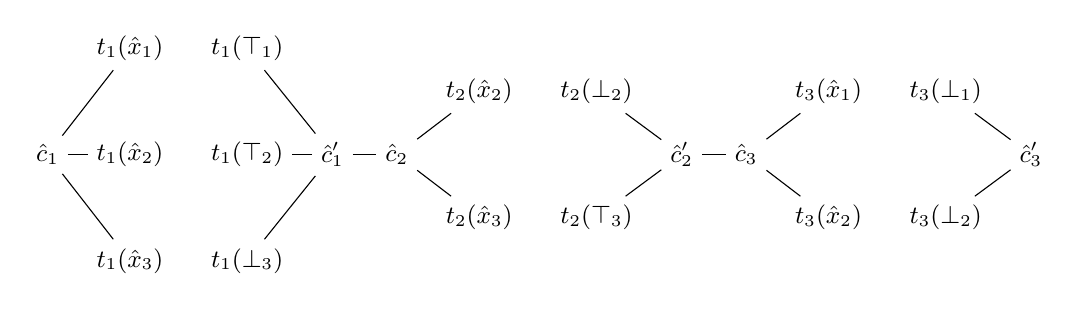
\begin{tikzpicture}[node distance=.3cm]
\small
\node(c1){$\hat{c}_1$};

\node[right =.25cm of c1] (t1x2) {$t_1(\hat{x}_2)$};
\node[above =.8cm of t1x2] (t1x1) {$t_1(\hat{x}_1)$};
\node[below =.8cm of t1x2] (f1x3) {$t_1(\hat{x}_3)$};
\draw [-] (c1) to (t1x2);
\draw [-] (c1) to (t1x1);
\draw [-] (c1) to (f1x3);

\node[right = 3.1cm of c1](c1p){$\hat{c}_1'$};

\node[left =.25cm of c1p] (t12) {$t_1(\top_2)$};
\node[above=.8cm of t12] (t11) {$t_1(\top_1)$};
\node[below=.8cm of t12] (f13) {$t_1(\bot_3)$};
\draw [-] (c1p) to (t11);
\draw [-] (c1p) to (t12);
\draw [-] (c1p) to (f13);

\node[right = .3cm of c1p](c2){$\hat{c}_2$};
\draw [-] (c1p) to (c2);

\node[right=.25cm of c2, yshift=.8cm]  (f2x2) {$t_2(\hat{x}_2)$};
\node[right=.25cm of c2, yshift=-.8cm] (t2x3) {$t_2(\hat{x}_3)$};
\draw [-] (c2) to (f2x2);
\draw [-] (c2) to (t2x3);

\node[right = 3.1cm of c2](c2p){$\hat{c}_2'$};
\node[left =.25cm of c2p, yshift=.8cm]  (f22) {$t_2(\bot_2)$};
\node[left =.25cm of c2p, yshift=-.8cm] (t23) {$t_2(\top_3)$};
\draw [-] (c2p) to (t23);
\draw [-] (c2p) to (f22);

\node[right = .3cm of c2p](c3){$\hat{c}_3$};
\draw [-] (c2p) to (c3);
\node[right =.25cm of c3, yshift=.8cm] (f3x1) {$t_3(\hat{x}_1)$};
\node[right =.25cm of c3, yshift=-.8cm] (f3x2) {$t_3(\hat{x}_2)$};
\draw [-] (c3) to (f3x1);
\draw [-] (c3) to (f3x2);

\node[right = 3.1cm of c3](c3p){$\hat{c}_3'$};
\node[left =.25cm of c3p, yshift=.8cm] (f31) {$t_3(\bot_1)$};
\node[left =.25cm of c3p, yshift=-.8cm] (f32) {$t_3(\bot_2)$};
\draw [-] (c3p) to (f31);
\draw [-] (c3p) to (f32);

\end{tikzpicture}


\caption{The congruence translation $E_{\mathcal{C}} = \Connect \cup \bigcup_{1 \leq i \leq n}\Clause_i$ of $\mathcal{C}$.}
\label{fig:npexamplebig}
\end{figure}

\end{example}

Assignments can also be translated to sets of equations:
\begin{definition}[Assignment congruence translation]
Let $\mathcal{I}$ be an assignment on variables $x_1,\ldots,x_m$.
%The set of terms $\mathcal{T}$ is constructed using the following constants and function symbols.
%For every $i= 1,\ldots,n + 1$, there is a constant $\hat{c}_i$ and function symbols $t_i$ and $f_i$.
%For every $j= 1,\ldots,m$, there are constants $\hat{x}_j$, $\top_j$ and $\bot_j$.
The congruence translation $E_{\mathcal{I}}$ of $\mathcal{I}$ is defined as the set of equations
\begin{eqnarray*}
  E_{\mathcal{I}} & = & \phantom{\cup}\ \{ \hat{x}_j = \top_j \ \mid\  1 \leq j \leq m \text{ and } \mathcal{I} \models x_j \} \\
               &   & \cup\ \{ \hat{x}_j = \bot_j \ \mid\ 1 \leq j \leq m \text{ and } \mathcal{I} \models \neg x_j \}
\end{eqnarray*}
For convenience, we also define the set
\begin{equation*}
  \Assignment^\star = \{ \hat{x}_j = \top_j, \hat{x}_j = \bot_j \ \mid\ 1 \leq j \leq m\}.
\end{equation*}
\end{definition}
\noindent
The congruence translation of an assignment is always a subset of
$\Assignment^\star$.  By abuse of language, a subset of $\Assignment^\star$ is
said to be an assignment if it is the congruence translation of an assignment,
that is, if it does not contain both $\hat{x}_j = \top_j$ and $\hat{x}_j =
\bot_j$ for some $j$.

\begin{example}\label{ex:np2} (Example~\ref{ex:np1} continued)  
Consider the model $\mathcal{I} = \{x_1, \neg x_2, x_3\}$ of\/ $\mathcal{C}$.
Figure~\ref{fig:npassignment} gives a graphical representation of
$E_{\mathcal{I}}$, whereas $\Assignment^\star$ is described by
Figure~\ref{fig:npassignmentstar}.  Notice that
$E_{\mathcal{C}} \cup E_{\mathcal{I}} \models \hat{c}_1 = \hat{c}'_3$,
and $\hat{c}_1$ and $\hat{c}'_3$ are connected in the congruence graph
of $E_{\mathcal{C}} \cup E_{\mathcal{I}}$ (Figure~\ref{fig:npmodel}).
This is actually the aim of the construction.

\begin{figure}[ht]

\centering
\begin{tikzpicture}[node distance=1.5cm]

\node [below =.5cm of f2x2] (x1) {$\hat{x}_1$};
\node [below =.5cm of x1] (x2) {$\hat{x}_2$};
\node [below =.5cm of x2] (x3) {$\hat{x}_3$};

\node [right = of x1] (t1) {$\top_1$};

\draw [-] (x1) to (t1);

\node [left = of x2] (f2) {$\bot_2$};

\draw [-] (x2) to (f2);

\node [right = of x3] (t3) {$\top_3$};

\draw [-] (x3) to (t3);

\end{tikzpicture}


\caption{Congruence translation of $\mathcal{I}$}
\label{fig:npassignment}
\end{figure}

\begin{figure}[ht]

\centering
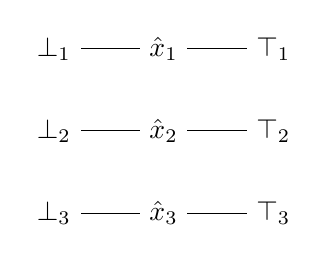
\begin{tikzpicture}[node distance=.75cm]

\node (x1) {$\hat{x}_1$};
\node [below =.5cm of x1] (x2) {$\hat{x}_2$};
\node [below =.5cm of x2] (x3) {$\hat{x}_3$};

\node [right = of x1] (t1) {$\top_1$};
\node [left = of x1] (f1) {$\bot_1$};

\draw [-] (x1) to (t1);
\draw [-] (x1) to (f1);

\node [right = of x2] (t2) {$\top_2$};
\node [left = of x2] (f2) {$\bot_2$};

\draw [-] (x2) to (t2);
\draw [-] (x2) to (f2);

\node [right = of x3] (t3) {$\top_3$};
\node [left = of x3] (f3) {$\bot_3$};

\draw [-] (x3) to (t3);
\draw [-] (x3) to (f3);

\end{tikzpicture}



\caption{$\Assignment^\star$}
\label{fig:npassignmentstar}
\end{figure}
\begin{figure}[ht]

\centering
\begin{tikzpicture}[node distance=.3cm]
\small
\node(c1){$\hat{c}_1$};

\node[right =.25cm of c1] (t1x2) {$t_1(\hat{x}_2)$};
\node[above =.8cm of t1x2] (t1x1) {$t_1(\hat{x}_1)$};
\node[below =.8cm of t1x2] (t1x3) {$t_1(\hat{x}_3)$};
\draw [-] (c1) to (t1x2);
\draw [-] (c1) to (t1x1);
\draw [-] (c1) to (t1x3);

\node[right = 3.1cm of c1](c1p){$\hat{c}_1'$};

\node[left =.25cm of c1p] (t12) {$t_1(\top_2)$};
\node[above=.8cm of t12] (t11) {$t_1(\top_1)$};
\node[below=.8cm of t12] (t13) {$t_1(\bot_3)$};
\draw [-] (c1p) to (t11);
\draw [-] (c1p) to (t12);
\draw [-] (c1p) to (t13);

\node[right = .3cm of c1p](c2){$\hat{c}_2$};
\draw [-] (c1p) to (c2);

\node[right=.25cm of c2, yshift=.8cm]  (t2x2) {$t_2(\hat{x}_2)$};
\node[right=.25cm of c2, yshift=-.8cm] (t2x3) {$t_2(\hat{x}_3)$};
\draw [-] (c2) to (t2x2);
\draw [-] (c2) to (t2x3);

\node[right = 3.1cm of c2](c2p){$\hat{c}_2'$};
\node[left =.25cm of c2p, yshift=.8cm]  (t22) {$t_2(\bot_2)$};
\node[left =.25cm of c2p, yshift=-.8cm] (t23) {$t_2(\top_3)$};
\draw [-] (c2p) to (t23);
\draw [-] (c2p) to (t22);

\node[right = .3cm of c2p](c3){$\hat{c}_3$};
\draw [-] (c2p) to (c3);
\node[right =.25cm of c3, yshift=.8cm] (t3x1) {$t_3(\hat{x}_1)$};
\node[right =.25cm of c3, yshift=-.8cm] (t3x2) {$t_3(\hat{x}_2)$};
\draw [-] (c3) to (t3x1);
\draw [-] (c3) to (t3x2);

\node[right = 3.1cm of c3](c3p){$\hat{c}_3'$};
\node[left =.25cm of c3p, yshift=.8cm] (t31) {$t_3(\bot_1)$};
\node[left =.25cm of c3p, yshift=-.8cm] (t32) {$t_3(\bot_2)$};
\draw [-] (c3p) to (t31);
\draw [-] (c3p) to (t32);

\node [below =1.3cm of c2, xshift=1.5cm] (x1) {$\hat{x}_1$};
\node [below =.5cm of x1] (x2) {$\hat{x}_2$};
\node [below =.5cm of x2] (x3) {$\hat{x}_3$};

\node [right = of x1] (t1) {$\top_1$};

\draw [-] (x1) to (t1);

\node [left = of x2] (t2) {$\bot_2$};

\draw [-] (x2) to (t2);

\node [right = of x3] (t3) {$\top_3$};

\draw [-] (x3) to (t3);

\draw [dotted] (t1x1) to (t11);
\draw [dotted] (t1x3) to (t13);
\draw [dotted] (t2x2) to (t22);
\draw [dotted] (t2x3) to (t23);
\draw [dotted] (t3x2) to (t32);

\end{tikzpicture}


\caption{The congruence graph for $E_{\mathcal{C}} \cup E_{\mathcal{I}}$}
\label{fig:npmodel}
\end{figure}
\end{example}

\begin{lemma}
\label{lemma:eqv}
Consider a (partial or total) assignment $\mathcal{I}$ for a set of clauses
$\mathcal{C}= \{C_1, \dots C_n\}$.  $\mathcal{I} \models \mathcal{C}$ if and only if
$E_{\mathcal{I}} \cup E_\mathcal{C} \models \hat{c}_1 = \hat{c}'_n$.
\end{lemma}
\begin{proof}
The condition is sufficient.  Consider the congruence graph induced by
$E_{\mathcal{I}} \cup E_\mathcal{C}$.  Besides edges directly associated to
equalities in the set, the only edges are congruence edges between terms
$t_i(\hat{x}_j)$ and either $t_i(\top_j)$ or $t_i(\bot_j)$.  So any path from
$\hat{c}_1$ to $\hat{c}_n$ would go through such a congruence edge for each $i$.
And such an edge exists for $i$ if and only if clause $i$ is satisfied by
$\mathcal{I}$.

The condition is also necessary.  If $\mathcal{I} \models \mathcal{C}$, then
$\mathcal{I} \models C_i$ for each clause $C_i \in \mathcal{C}$.  Assume
$\mathcal{I}$ makes true a variable $x_j$, literal of $C_i$ (the case of
the negation of a variable is handled similarly).  Then $E_{\mathcal{I}} \models
t_i(\hat{x}_j) = t_i(\top_j)$, and $E_{\mathcal{I}} \cup \Clause_i
\models \hat{c}_i = \hat{c}_i'$.  This is true for each $i$, and
thanks to the equations in \Connect, one can deduce using transitivity that
$E_{\mathcal{I}} \cup E_\mathcal{C} \models \hat{c}_1 = \hat{c}_n'$.
\end{proof}

\noindent Notice also that, for any model $\mathcal{I}$ of a set of $n$ clauses
$\mathcal{C}$, every explanation that $E_{\mathcal{I}} \cup E_\mathcal{C}
\models \hat{c}_1 = \hat{c}_n'$ contains at least two equalities in
each set $\Clause_i$, since each clause has to be satisfied.  But also, there is
an explanation that contains exactly two equalities in each set $\Clause_i$.
Considering again Example~\ref{ex:np2}, and particularly
Figure~\ref{fig:npmodel}, any transitivity chain from $\hat{c}_1$ to
$\hat{c}'_3$ will pass through $\hat{c}'_1$, $\hat{c}_2$, $\hat{c}_2'$ and
$\hat{c}_3$.  Any acyclic path from $\hat{c}_1$ to $\hat{c}'_3$ will contain 11
edges: 3 congruence edges, $3\times 2$ edges in $\Clause_i$ for $i=1,\dots 3$
and 2 edges from $\Connect$.

Since every interpretation $\mathcal{I}$ is such that $E_{\mathcal{I}} \subset
\Assignment^\star$, one can try to relate the propositional satisfiability
problem for a set of clauses $\mathcal{C}= \{C_1, \dots C_n\}$ to finding an
explanation of $\hat{c}_1 = \hat{c}_n'$ in $\Assignment^\star \cup
E_{\mathcal{C}}$.  However, it is necessary that this explanation does not set
$\hat{x}_j$ equal both to $\top_j$ and $\bot_j$, i.e.\ at most one of the two
equations $\hat{x}_j = \top_j$ and $\hat{x}_j = \bot_j$ should be in the
explanation.  By restricting assignments to total ones, i.e.\ by enforcing that
at least one of the two equations $\hat{x}_j = \top_j$ and $\hat{x}_j = \bot_j$
belongs to the explanation, it is also possible, with a single cardinality
constraint on the explanation, to require that at most one of them belong to the
explanation.


\begin{lemma}
A set of clauses $\mathcal{C}= \{C_1, \dots C_n\}$ using variables $x_1,\dots
x_m$ is satisfiable if and only if there is a subset $E' \subseteq
\Assignment^\star \cup E_{\mathcal{C}'}$ such that $E'\models \hat{c}_1 =
\hat{c}'_{n+m}$ and $|E'| \leq 3n+4m-1$, where $\mathcal{C}'$ is $\mathcal{C}$
augmented with the tautological clauses $c_{n+i} = x_i \vee \neg x_i$ for
$i=1,\dots m$.
\end{lemma}
\begin{proof}
The condition is straightforwardly necessary.  It is also sufficient since an
explanation of $\hat{c}_1 = \hat{c}'_{n+m}$ has to contain $2(n + m)$
equations from $Clause_i$ ($i= 1\dots n + m$) and $n + m - 1$ equations from
$\Connect$.  Thanks to the tautological clauses, any explanation also has to
contain at least $\hat{x}_j = \top_j$ or $\hat{x}_j = \bot_j$ for each
$j\in\{1\dots m\}$. Therefore, the cardinality constraint requires that the explanation
contains at most one $\hat{x}_j = \top_j$ or $\hat{x}_j = \bot_j$ for each
$j\in\{1\dots m\}$.  If such an explanation exists, Lemma~\ref{lemma:eqv}
guarantees the existence of a model for $\mathcal{C'}$, or equivalently for
the original set of clauses $\mathcal{C}$.
\end{proof}




\begin{corollary}[NP-hardness]
\label{lemma:nphardness}
The small explanation problem is NP-hard.
\end{corollary}
\begin{proof}
Propositional satisfiability is NP-hard, and can be reduced in polynomial time
to the small explanation problem.
\end{proof}

\begin{lemma}[NP]
\label{lemma:innp}
The small explanation problem is in NP.
\end{lemma}
\begin{proof}
A solution to the small explanation decision problem is a subset of the input
equations, therefore it is clearly polynomial in the problem size.  Whether
a subset $E'$ is a solution can be verified by computing its congruence closure
and checking whether the target equation $s = t$ is implied. Congruence closure can be computed in polynomial time
\cite{Nelson2,Downey1,Nieuwenhuis6}.
\end{proof}


\begin{theorem}[NP-completeness]
The small explanation problem is NP-complete.
\end{theorem}
\begin{proof}
By lemmas~\ref{lemma:nphardness} and~\ref{lemma:innp}.
\end{proof}

\begin{theorem}[NP-completeness]
The small conflict set problem is NP-complete.
\end{theorem}
\begin{proof}
The small conflict set problem is at least as hard as the small explanation problem since the small explanation problem has been showed to be reducible to the small conflict set problem.  It is also in NP for exactly the same reason that the small explanation problem is.
\end{proof}


\section*{Conclusion}

\marginpar{Besson PxTP}
The extraction of small explanations for the congruence of terms is an interesting subroutine of the classical congruence closure algorithm, which is especially relevant in applications where proofs are desirable. When the lack of solution for an unsatisfiable problem needs to be externally verified, a proof/refutation may serve as a certificate of the unsatisfiability.

We have shown that the problem of deciding whether an explanation of a given size exists is NP-complete. Therefore, it is generally intractable to obtain the smallest explanation. 

In \cite{Nieuwenhuis3,Nieuwenhuis9} methods to obtain small, but not necessary the smallest, explanations are discussed.
However, the proof tree data structure used in those methods is designed to prioritize speed of the congruence closure algorithm. 
Other methods prioritizing small size of extracted explanations could still be investigated. Thanks to the NP-completeness, one option would be to iteratively encode the small explanation problem into SAT, and use SAT-solvers to find succesively smaller explanations, until the smallest explanation is found. \marginpar{note that we would have to encode and call a SAT-solver many times, with progressively smaller values of $k$, until we find a value of $k$ for which the encoded problem is unsatisfiable. this would guarantee a \emph{minimum} conflict, but would probably be less efficient than the iterative addition/removal of literals from the explanation, which only guarantees a \emph{minimal} conflict.} 

\vspace*{5pt}\noindent
{\bf Acknowledgment.} We would like to thank Roberto Nieuwenhuis and Ashish
Tiwari for discussions and some preliminary ideas that led us to this proof.

\bibliographystyle{plain}
\bibliography{biblio}

\end{document}
